\documentclass[12pt, a4paper]{article}
\usepackage{graphicx}
\usepackage{mathtools}
\usepackage{xcolor}
\usepackage{amsmath}
\usepackage{caption}
\usepackage[italian]{babel}
\usepackage{setspace}
\usepackage{geometry}
\graphicspath{ {./immagini/} }
\linespread{1.1}
\geometry{
 total={170mm,257mm},
 left=20mm,
 top=15mm,
 bottom=28mm
 }
 
 \title{\textbf{\scalebox{1.3}{\text{Moto di un grave lungo la verticale}}}}
 \date{}

\author{\begin{small}Mussini Simone, Ruscillo Fabio, Musi Francesco\end{small}}



\begin{document}
\maketitle
\section{Obbiettivo}
Lo scopo di questo esperimento è di riuscire ad ottenere la misura dell'accelerazione di gravità, analizzando un filmato che ritrae una sferetta in caduta libera. 
Ciò è stato fatto prendendo varie misure della posizione del corpo tramite fotoregistrazioni ad alta velocità. 
La formula che mette in relazione la posizione del corpo e $g$ è:
\begin{equation*}
    y(t) = \frac{1}{2}gt^2
\end{equation*}


\section{Strumenti}
\begin{itemize}
\setlength\itemsep{0mm}
    \item Programma di analisi "Tracker"
    \item Video con 1000 fotogrammi al secondo
\end{itemize}

\section{Procedimento di misura}
Il setup del video comprende un asta metallica alla sommità della quale è posizionata una sferetta metallica ferma. L'asta presenta dei segni distanziati di 10cm. 
Ad un certo punto la sferetta viene rilasciata. Affianco all'asta è presente un cronometro con sensibilità al millesimo di secondo. 
Essendo il tutto filmato da una fotocamera (Sony DSC-RX100M4) che registra a 1000fps, ad ogni frame il cronometro avanza di un millesimo di secondo.

  
\subsection{Setting del programma di tracciamento}
Per iniziare, mediante la funzione "asta di calibrazione" si è posto uguale a 10cm la distanza tra 2 segni sull'asta, in modo che il programma potesse generare un metro calibrato con cui misurare la posizione del target. \\
Poi si è stabilito il frame di inizio del moto, che è risultato essere il 49esimo.  \\
La posizione è stata tracciata ogni 10 frame, mettendo i punti di massa nella parte inferiore della sferetta. Il metro calibrato è stato posto sulla schermata in modo che coincidesse con la posizione del punto di massa a target fermo.\\
In totale sono state prese 41 misure.


\subsection{Gestione degli errori}
L'alta velocità di acquisizione della fotocamera è a scapito della quantità di luce catturata, quindi anche della nitidezza dell'immagine. Per questo è stato necessario stimare ogni grandezza tramite un errore. \\
Gli errori sono stati misurati in base al numero di pixel di transizione tra il colore del target e dello sfondo, e sono stati stimati misura per misura visto che la chiarezza di ogni frame era variabile. Tramite il metro di calibrazione, è stato posto: 1$px$ = 0.0005$m$, pertanto
\begin{equation*}
    \Delta y_{misurato}= (\Delta pixel \cdot 0.0005)m
\end{equation*}
\bigskip
Tutte le misure sono state riportate in Tabella \ref{Tabella Completa}

\section{Analisi dei dati}
Il frame di inizio della caduta è il 49esimo, che corrisonde ad un tempo iniziale \textit{$t_i = 0.012s$}.
Abbiamo poi terminato lo studio del moto al 459esimo fotogramma, che corrisponde all'istante \textit{$t_f = 0.422s$}, per un tempo totale di caduta \textit{$\Delta t = 0.410s$}. 
E' stato scelto come ultimo istante di caduta, quello che corrisponde all'ultima misura utile, appena precedente al rimbalzo della pallina sul banco di lavoro.\\

Successivamente siamo passati al calcolo degli errori relativi di $y$ e $t$, per stabilire quale tra le due è la variabile dipendente e quale quella idipendente. Ciò che si è riscontrato è che esse hanno lo stesso ordine di grandezza, pertanto calcoliamo un nuovo errore su $y$ pari a 
\begin{equation*}
   \Delta y^{'} = \left(\frac{2\Delta t}{t}\right)\cdot y + \Delta y_{misurato}
\end{equation*}
\subsection{Grafico spazio-tempo}
Il primo grafico realizzato con il programma di analisi dati \textit{Igor Pro} è stato il grafico spazio-tempo, ossia quello della legge oraria, che dovrebbe seguire la formula indicata nel primo paragrafo (traiettoria parabolica con posizione e velocità iniziali nulle).\\ 
Sulle ordinate compaiono i valori numerici di \textit{y(t)}, associati ai relativi errori  \textit{$\Delta y^{'}$}, mentre sulle ascisse ci sono gli istanti di tempo \textit{t}. 

I dati ottenuti tramite la regressione di potenza del secondo ordine (\textit{poli 3}), non sono compatibili con i valori teorici, fatta eccezione per $\displaystyle{\frac{g}{2}}$ :


\renewcommand{\theenumii}{\roman{enumii}}  
\begin{itemize}
    \itemsep0em 
    
        \item Posizione iniziale $y(0)$:
        
        \begin{tabular}{ccc}
        {$K_0 = -0.0010852 \pm 0.000739$} & & \small{(Non compatibile con il valore atteso $K_{0}$ $_{atteso}= 0.0000$)}\\
        \end{tabular}
        
    \end{itemize}
    \begin{itemize}
        \item Velocità iniziale $v(0)$:\\
        \begin{tabular}{ccccc}
        {$K_1 =  0.020001 \pm 0.0128$} & & & & \small{(Non compatibile con il valore atteso $K_{1}$ $_{atteso} = 0.0000$)}\\
        \end{tabular}
        
    \end{itemize}
      \begin{itemize}
          \item Coefficiente del termine quadratico, pari a $\displaystyle{\frac{g}{2}}$:\\ 
          \begin{tabular}{cccccc}
              {$K_2 =  4.9298 \pm 0.0353$} & & & & &\small{(Compatibile con il valore atteso $K_{2}$ $_{atteso}= 4.9033$)}\\
          \end{tabular}
         
      \end{itemize}
        
        
\newpage

Visto che \textit{posizione iniziale} e \textit{velocità iniziale} non sono compatibili con i valori attesi abbiamo corretto l'incompatibilità, isolando a destra il termine in relazione  quadratica con il tempo, mentre a sinistra, abbiamo ottenuto una nuova variabile $y_{new}$ in cui la posizione è corretta dai termini $K_0$ e $ K_1\ t$, col rispettivo errore $\Delta y_{new}$: \\
L'equazione diventa quindi:
\begin{equation*}
\begin{aligned}
  & & y - K_0 - K_1\ t = K_0'+K_1'\ t+K_{2}'\ t^2
  &\quad{} 
  \end{aligned}
  \begin{aligned}
  & &\text{dove:\phantom{.......}} y_{new} = y - K_0 - K_1\ t 
  &
  \end{aligned}
\end{equation*}
L'errore su  $y_{new}$ è dato da
\begin{equation*}
 \Delta y_{new} = \Delta y + \Delta K_0 + \sqrt{\left(\frac{\Delta K_1}{K_1}\right)^2 + \left(\frac{\Delta t}{t}\right)^2}
 \end{equation*}
Facendo una nuova regressione di potenza del secondo ordine utilizzando i nuovi dati, otteniamo che le variabili $K_0'$, $K_1'$ e $K_2'$ sono tutte compatibili, come possiamo vedere in Figura \ref{Grafico parabolico}:
\bigskip
\bigskip

    \begin{figure}[h]
\centering
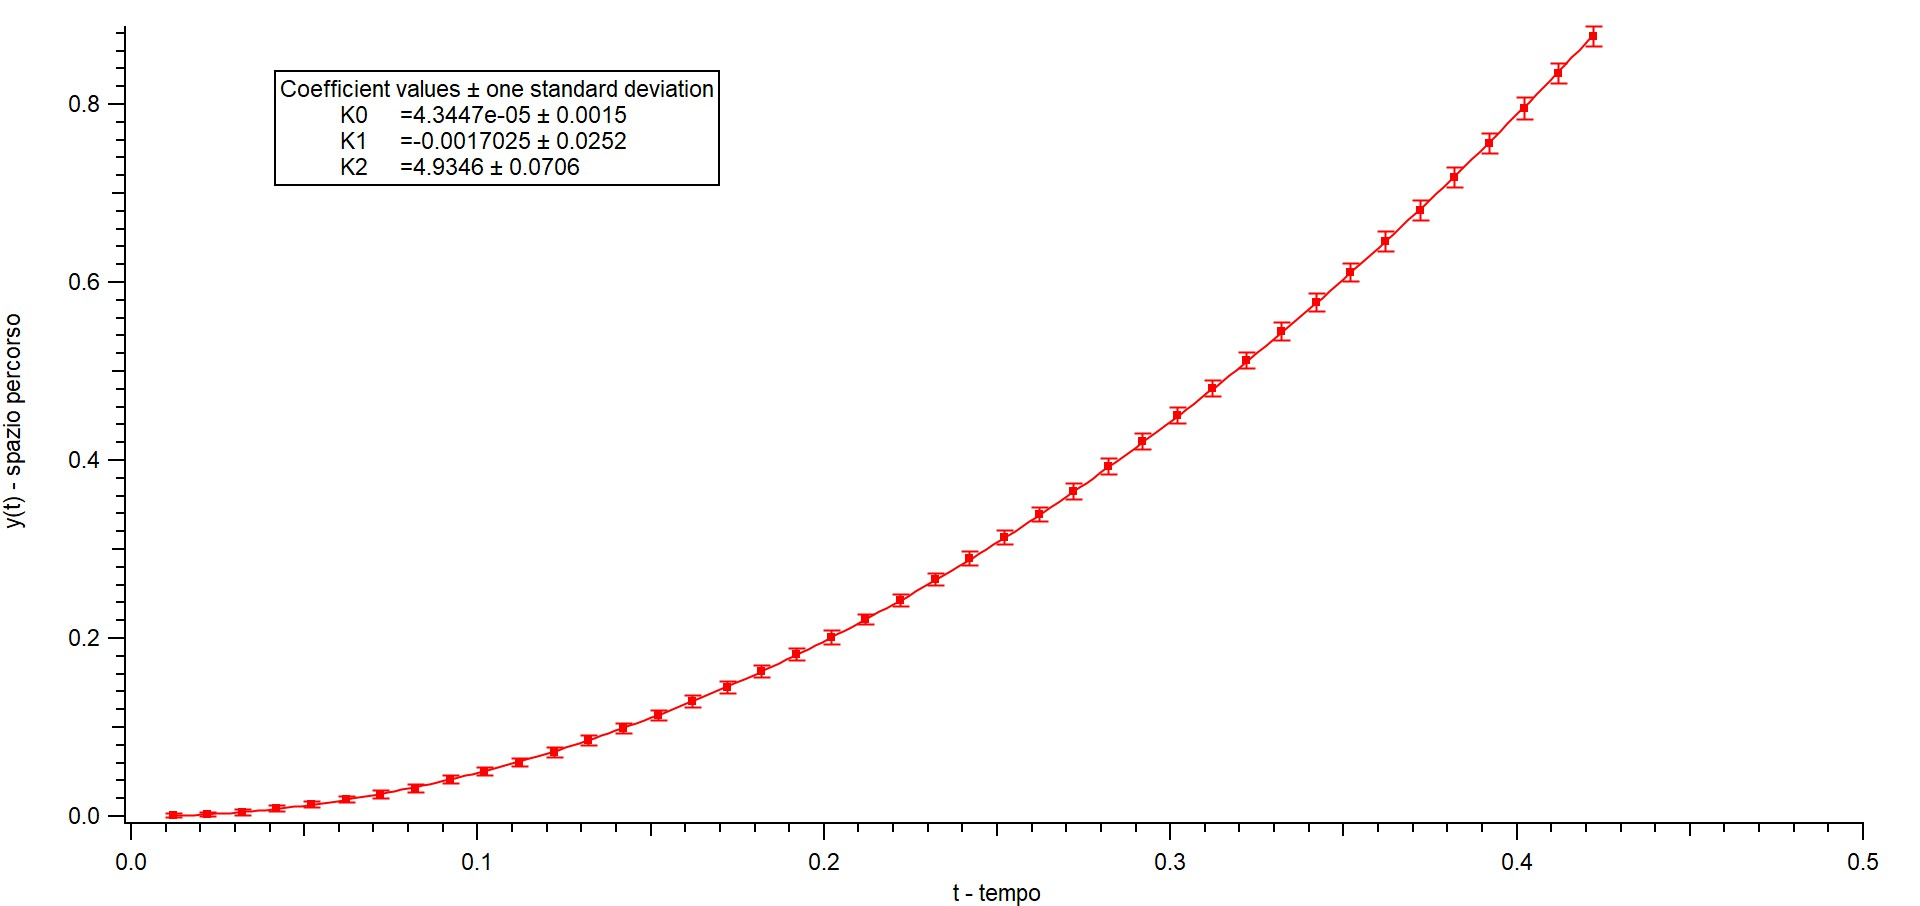
\includegraphics[width=170mm]{Immagini/Graph1.jpg}
\caption{\textit{{\footnotesize{Grafico $y_{new}(t)$: sul'asse asse $y$ sono riportati i valori di $y_{new}$ coi rispettivi errori, sull'asse $x$ il tempo}}}}
\label{Grafico parabolico}
\end{figure}

\section{Regressione lineare}
Successivamente si è fatta una regressione lineare, partendo da $y_{new}= \frac{1}{2}\ g t^2$, approssimando posizione e velocità iniziali a $0$. Quello che ci si aspetta di trovare è che la posizione sia in relazione quadratica con il tempo:
\begin{equation*}
\begin{aligned}
  & y_{new}= \frac{1}{2}\ g\ t^2
  &\quad{} 
  \end{aligned}
  \begin{aligned}
  &&\text{passando ai logaritmi:\phantom{..}}& & \ln(y_{new})=\ln\left({\frac{1}{2}\ g}\right) +2\ln{t}
  &
  \end{aligned}
\end{equation*}
e come errore su $\ln({y_{new}})$: 
\begin{equation*}
    \Delta\ln{(y_{new})}=\frac{\Delta y_{new}}{y_{new}}\ 
\end{equation*}\\
 Tramite \textit{Igor Pro} si è ottenuto il seguente grafico:\\
   \begin{figure}[h!]
\centering
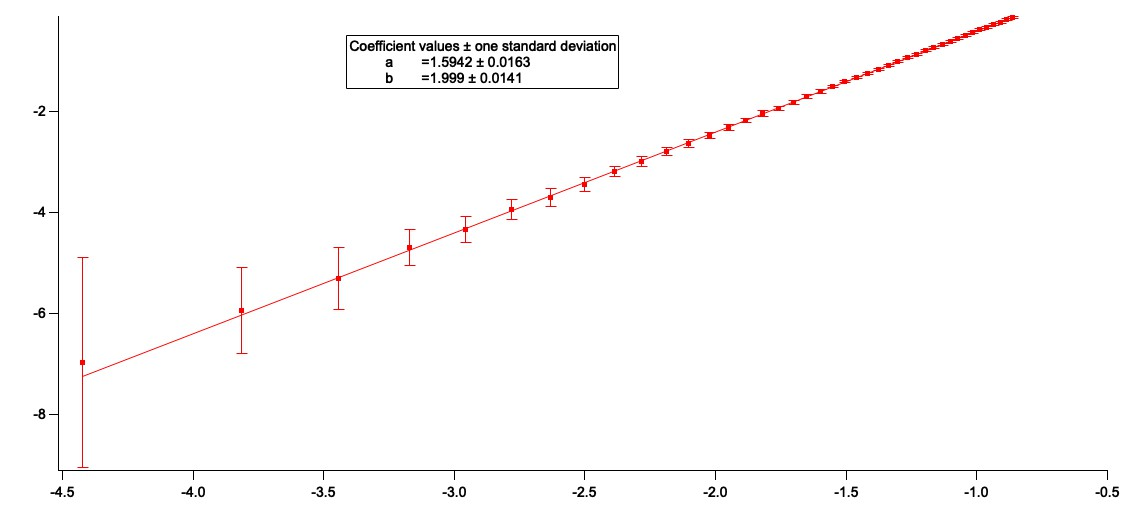
\includegraphics[width=170mm]{Immagini/GraphLn.jpg}
\caption{\textit{{\footnotesize{Grafico $\ln{(y_{new})}(\ln{t})$: sul'asse asse $y$ sono riportati i valori di $\ln{(y_{new)}}$ coi rispettivi errori, sull'asse $x$ il logaritmo del tempo}}}}
\label{Grafico logaritmico}
\end{figure}

Il valore di $b$ è compatibile col valore $2$, esponente del tempo nella formula usata in partenza.  Si è così dimostrato che vi è una relazione quadratica tra $y_{new}$ e $t$.



\section{Calcolo dell'accelerazione di gravità}
A questo punto, dopo aver verificato che la posizione iniziale e finale sono approssimabili a $0$, e che la poszione è in relazione quadrtica con il tempo, possiamo creare un grafico lineare dei valori $y_{new}$, coi rispettivi errori, e del tempo al quadrato, così da essere in grado di ricavare il valore dell'accelerazione di gravità. L'intercetta e la pendenza della retta ottenuta sono:
\begin{itemize}
    \item $a=-3.691\cdot 10^{-5}\pm 0.000921$
    \item$b=4.9301\pm 0.0216$
\end{itemize}
Dove $b=\frac{1}{2}\ g=(4.9301\pm 0.0216)$, da cui:
\begin{equation*}
    g=2 \ b=9.8602
\end{equation*}
e l'errore è
\begin{equation*}
    \Delta g=2\ \Delta b=0.04
\end{equation*}
Quindi l'accelerazione di gravità ottenuta sarebbe $g=(9.86\pm0.04)$ $\frac{m}{s^2}$.
Il valore $g$, ricavato a partire da $b$ , non risulta compatibile col valore tabulato. Questo è dovuto al fatto che ci potrebbero essere errori risultanti dalla configurazione e dalla qualità video dell'esperimento, che non erano sotto il nostro controllo. Per queste ragioni si è passati a due deviazioni standard con una confidenza del 95\%, e il grafico ottenuto è il seguente:
  \begin{figure}[h!]
\centering
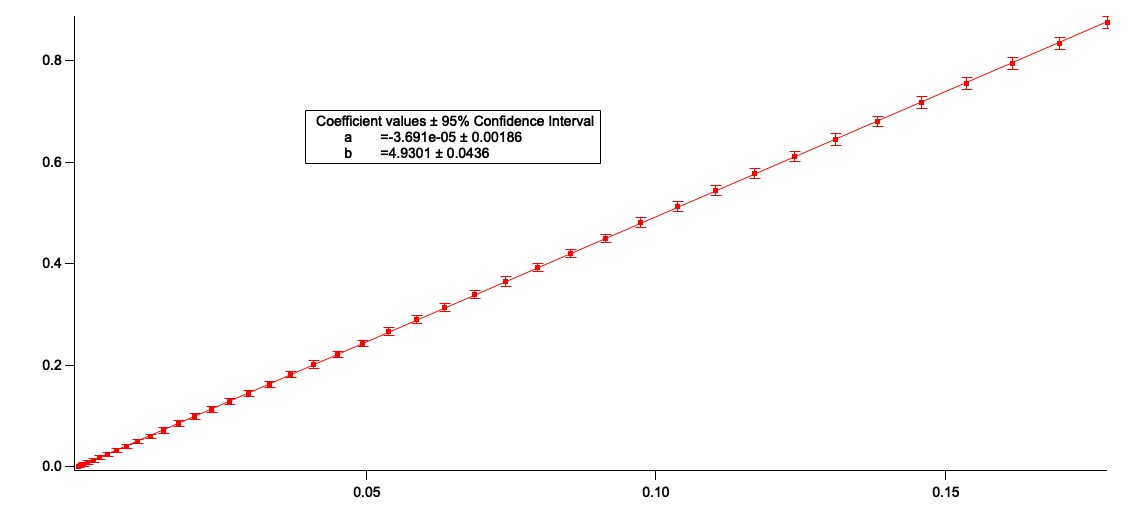
\includegraphics[width=170mm, height=80mm]{Immagini/Graphy_t^2.jpg}
\caption{\textit{{\footnotesize{Grafico $y_{new}(t^2)$: sul'asse asse $y$ sono riportati i valori di $y_{new}$ coi rispettivi errori, sull'asse $x$ il tempo al quadrato}}}}
\label{Grafico logaritmico}
\end{figure}

Si è infine passati al calcolo di $g$, utilizzando il valore di $b$ con un nuovo errore:
\begin{equation*}
    g=2 \ b=9.8602
\end{equation*}
e l'errore è
\begin{equation*}
    \Delta g=2\ \Delta b=0.08
\end{equation*}
Quindi il valore dell'accelerazione di gravità è $g=(9.86\pm0.08)$ $\frac{m}{s^2}$, compatibile col valore tabulato.



\newpage

\section{Tabella completa}
\begin{table}[h!]
    \centering
    {\renewcommand\arraystretch{1.0} 
    \begin{tabular}{|c|c|c|c|}
    \hline
         \footnotesize Misura & $y$$(m)$ &$\Delta pixel$& $\Delta y_{misurato}$ \\
    \hline
         \footnotesize 1 &\footnotesize 0.0001& & \\
         \footnotesize 2 & \footnotesize0.0020& & \\
         \footnotesize 3 & \footnotesize0.0045& & \\
         \footnotesize 4 & \footnotesize0.0090& & \\
         \footnotesize 5 & \footnotesize0.0130& & \\
         \footnotesize 7 &\footnotesize0.0195 & & \\
         \footnotesize 8 &\footnotesize0.0250 & & \\
         \footnotesize 9 & \footnotesize0.0325& & \\
         \footnotesize 10 &\footnotesize0.0420 & & \\
         \footnotesize 11 & \footnotesize0.0515& & \\
         \footnotesize 12 & \footnotesize0.0620& & \\ 
         \footnotesize 13 &\footnotesize 0.0730& & \\
         \footnotesize 14 & \footnotesize0.0865& & \\
         \footnotesize 15 & \footnotesize0.1005& & \\
         \footnotesize 16 & \footnotesize0.1160& & \\
         \footnotesize 17 & \footnotesize0.1315& & \\
         \footnotesize 18 & \footnotesize0.1475& & \\
         \footnotesize 19 & \footnotesize0.1660& & \\
         \footnotesize 20 & \footnotesize0.1850& & \\
         \footnotesize 21 & \footnotesize0.2045& & \\
         \footnotesize 22 &\footnotesize 0.2250& & \\
         \footnotesize 23 & \footnotesize0.2465& & \\
         \footnotesize 24 & \footnotesize0.2700& & \\
         \footnotesize 25 & \footnotesize0.2935& & \\
         \footnotesize 26 & \footnotesize0.3180& & \\
         \footnotesize 27 & \footnotesize0.3435& & \\
         \footnotesize 28 & \footnotesize0.3700& & \\
         \footnotesize 29 & \footnotesize0.3975& & \\
         \footnotesize 30 & \footnotesize0.4260& & \\
         \footnotesize 31 & \footnotesize0.4550& & \\ 
         \footnotesize 32 & \footnotesize0.4865& & \\
         \footnotesize 33 & \footnotesize0.5180& & \\
         \footnotesize 34 & \footnotesize0.5500& & \\
         \footnotesize 35 & \footnotesize0.6175& & \\
         \footnotesize 36 & \footnotesize0.6520& & \\
         \footnotesize 37 & \footnotesize0.6875& & \\
         \footnotesize 38 & \footnotesize0.7245& & \\
         \footnotesize 39 & \footnotesize0.7625& & \\
         \footnotesize 40 & \footnotesize0.8020& & \\
         \footnotesize 41 & \footnotesize0.8420& & \\
         \footnotesize 42 &\footnotesize 0.8835& & \\
    \hline
         
    \end{tabular}}
    \caption{Caption}
    \label{Tabella Completa}
\end{table}

\end{document}
